% Guard: macros.tex is \input both by main.tex (after the packages it needs,
% e.g. amsmath for \DeclareMathOperator) and by individual section files so
% they remain compilable on their own. Loading it twice would redefine every
% \newcommand and abort, so the second and later loads are no-ops.
\ifdefined\PQRmacrosloaded\endinput\fi
\let\PQRmacrosloaded\relax

% --- 0. revision marking ---
% Text added to Section 2 during the current revision is wrapped in \added{...}
% so the advisors can see at a glance what is new. Redefine to \relax to print
% the paper without the marking.
\newcommand{\added}[1]{\textcolor{blue}{#1}}
\long\def\added#1{\begingroup\color{blue}#1\endgroup}  % \long: may span paragraphs


% --- A. operator-style score and function names ---
\newcommand{\HD}{\mathit{HD}}                        % histogram distance; use \HD_\gamma
\newcommand{\Attr}{\mathit{Attr}}                    % attribute set of a schema
\newcommand{\Attrs}{\mathit{Attrs}}                  % attribute set argument
% Abbreviated in MATH only; the prose still spells the names out in full.
% Spelling them out inside formulas makes displayed equations far too wide
% for a two-column layout (the product-rule step below overflowed by 200pt).
\newcommand{\Use}{\mathit{Use}}
\newcommand{\Cov}{\mathit{Cov}}
\newcommand{\Rep}{\mathit{Rep}}
\newcommand{\DivS}{\mathit{Div}}
\newcommand{\TVD}{\mathit{TVD}}
\newcommand{\GS}{\mathit{GS}}                        % global sensitivity
\DeclareMathOperator{\Dom}{Dom}
\DeclareMathOperator{\Lap}{Laplace}

% --- B. core objects ---
\newcommand{\Qone}{Q_1}
\newcommand{\Qtwo}{Q_2}
\newcommand{\pD}{p(D)}
\newcommand{\views}{\mathcal{P}}
\newcommand{\hist}[2]{H_{#1,#2}}                     % \hist{\Qone(\pD)}{A}
\newcommand{\dhist}{\Delta H}
\newcommand{\nhist}{\widetilde{\Delta H}}            % the released noisy object

% --- C. privacy budget and parameters ---
\newcommand{\eps}{\epsilon}
\newcommand{\epsP}{\epsilon_P}
\newcommand{\epsS}{\epsilon_S}
\newcommand{\epsH}{\epsilon_H}
\newcommand{\gammaref}{\gamma_{\mathrm{ref}}}
\newcommand{\gammaeval}{\gamma_{\mathrm{eval}}}
\newcommand{\taumax}{\tau_{\max}}

% --- D. mechanisms ---
\newcommand{\ExpMech}{\textsc{ExpMech}}
\newcommand{\OneShotTop}[1]{\textsc{OneShotTop-}#1}
\newcommand{\AdaptiveTau}{\textsc{AdaptiveTau}}
% --- E. experiment baselines (used in sections/experiments.tex) ---
\newcommand{\Bone}{\ensuremath{\mathsf{B1}}}
\newcommand{\Btwo}{\ensuremath{\mathsf{B2}}}
\newcommand{\Bthree}{\ensuremath{\mathsf{B3}}}

\section{Problem Statement and Model}\label{sec:model}

This section states what an explanation is and what we are looking for (Section~\ref{subsec:private-query-difference-setting}), gives the measures of explanation quality as modifications of the forms used in prior work (Section~\ref{sec:explanation-quality}), bounds the sensitivity of each of them (Section~\ref{subsec:ideal-sensitivity}), and derives from that the two-stage structure the framework uses and the two utilities it optimises (Section~\ref{subsec:two-stages}).
\ag{Slightly overstated. Section~\ref{subsec:ideal-sensitivity} bounds the smoothed Histogram Distance and gives lower bounds for the three forms used in prior work, but it gives no bound for $\Rep_{\gamma_R}$ or $\Cov$ on its own, and the zero sensitivity of $\DivS$ is stated where $\DivS$ is defined. Suggest rephrasing to what it actually does, and likewise for the closing sentence of the Section~\ref{sec:explanation-quality} preamble.}

\subsection{Private Explanations of Query Differences}
\label{subsec:private-query-difference-setting}

We consider a trusted server that holds a private database $D$ and two related queries $Q_1$ and $Q_2$ over it.
The second query is typically derived from the first by a mechanism that the framework treats as a black box.
In query refinement (Definition~\ref{def:refinement}), $Q_1=Q$ is the original query and $Q_2=Q'$ its refinement; in consistent query answering (Definition~\ref{def:consistent-answer}), $Q_2$ is $Q_1$ evaluated under repair semantics.
Both are instances of the same problem, explaining how two related queries differ on the same database, and the framework does not depend on which one produced the pair.
For a view $p$ we write $Q_i(p(D))$ for the restriction of the output of $Q_i$ to the view, $Q_i(D)\cap p(D)$ (Section~\ref{subsec:prelim-settings}); for a selection query it is the result of evaluating $Q_i$ on $p(D)$ (Proposition~\ref{prop:view-restriction}).

Our goal is to let an analyst see \emph{how} the two outputs differ, which parts of the population the change added, removed or reshaped, while revealing nothing about any individual in $D$.
Two things have to be settled for that: what an explanation looks like, and what makes one good.
This subsection settles the first, and Section~\ref{sec:explanation-quality} the second; given those quality measures, the task is to return a handful of explanations that score well under them, privately.

\paragraph{Workflow.}
The analyst states what is to be explained and under what budget (Figure~\ref{fig:framework}): the two queries $Q_1$ and $Q_2$, the collection $\views$ of view predicates to search over, the explanation attributes $\Attrs$, the number of explanations $k$ and the privacy budget $\epsilon$.
Both queries are given.
How $Q_2$ was obtained, whether from a refinement algorithm, a repair procedure or the analyst writing it by hand, happens before the framework runs and is not part of it; the same holds for $\views$, which the analyst either supplies or has generated from the schema under the bound of Section~\ref{subsec:prelim-db-queries}.
Algorithm~\ref{alg:main} takes two further arguments, the reference smoothing constant $\gamma_R$ and the diversity weight $\lambda$.
These do not say what to explain; they tune how the two private stages trade accuracy against noise.
The two constants that matter most, how many views the first stage keeps and how hard the second stage smooths, the algorithm fixes for itself in Section~\ref{subsec:explanation-generation}.
The server then evaluates both queries, privately selects a small set of views from $\views$ and, within them, the explanation candidates that best characterise the difference, and releases noisy histograms for the selected candidates.
Only this last object leaves the server; the analyst never observes $D$, the exact outputs, or the exact scores that drove the selection.
Because $Q_2$ arrives as an input, the privacy analysis accounts for the explanation alone; if the mechanism that produced $Q_2$ read $D$, its own privacy cost composes with ours and is outside our scope.
\alon{Done: trusted-server workflow described above and depicted in Figure~\ref{fig:framework}.}

\begin{figure*}[t]
\centering
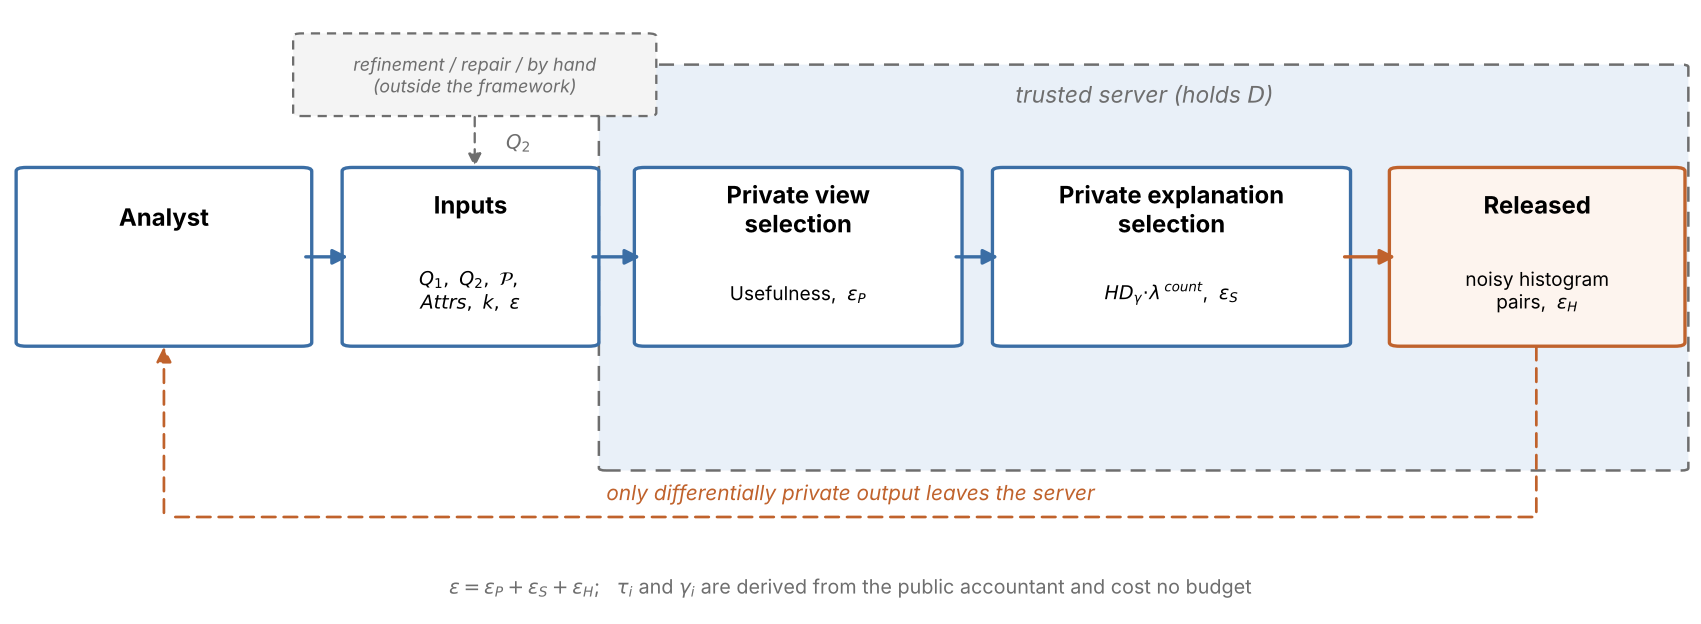
\includegraphics[width=\linewidth]{figures/framework.png}
\caption{The private query-difference explanation framework.
The analyst supplies both queries together with the search space and the budget; where $Q_2$ came from, whether a refinement algorithm, a repair procedure or the analyst, is outside the framework.
The server privately selects views, then explanations, and releases only noisy histogram pairs.
The constants $\tau$ and $\gamma$ are fixed from public quantities and therefore consume no budget.}
\label{fig:framework}
\end{figure*}

\paragraph{The structure of an explanation.}
An explanation answers \emph{where} the two outputs differ and \emph{in what respect}.
The where is a region of the database, given by a view predicate $p\in\views$; the respect is an attribute $A\in\Attrs$, whose distribution the two outputs are compared on.

\begin{definition}[Histogram Explanation Candidate]
\label{def:candidate}
Given a view $p\in\views$ and an explanation attribute $A\in\Attrs$, the \emph{histogram explanation candidate} $e=(p,A)$ induces the two histograms
\[
    \hist{Q_1(\pD)}{A}
    \qquad\text{and}\qquad
    \hist{Q_2(\pD)}{A}.
\]
Writing $\mathrm{attr}(p)$ for the attributes the predicate $p$ constrains, the space of candidates is
\[
\mathcal{C}=\{(p,A)\in\views\times\Attrs \;:\; A\notin\mathrm{attr}(p)\},
\]
and we write $E\subseteq\mathcal{C}$ for a set of them.
\ag{$\mathcal{C}$ already denotes the output-constraint set in Definitions~\ref{def:output-constraint} and~\ref{def:refinement}, both cited earlier in this section. Suggest renaming one of the two, for instance $\mathcal{E}$ for the candidate space here.}
A view that fixes $A$ leaves the two histograms supported on a single bin, so such a pair reports the change in one count rather than a change in a distribution; excluding it also keeps the candidate space aligned with the reference set of Section~\ref{sec:explanation-quality}, from which $\mathrm{attr}(p)$ is excluded for the same reason.
\end{definition}

\begin{example}[Explanation candidates]
\label{ex:candidate}
Figure~\ref{fig:candidates} shows two candidates for the refinement of Example~\ref{ex:running}, both on $A=\texttt{occupation}$.
In panel (a) the view is $p=(\texttt{education}=\texttt{Masters})$: both queries meet it, and the refinement shifts the occupational mix towards professional-specialty roles rather than merely adding people.
In panel (b) the view is $p'=(\texttt{education}=\texttt{Bachelors})$, which $\varphi_2$ cannot satisfy, so $Q_2(p'(D))=\emptyset$ and the candidate reports a population the refinement removes in its entirety.
Neither change is visible in the aggregate value, and the second is the kind of one-sided view the measures of Section~\ref{sec:explanation-quality} have to handle rather than discard.
\end{example}

\begin{figure*}[t]
\centering
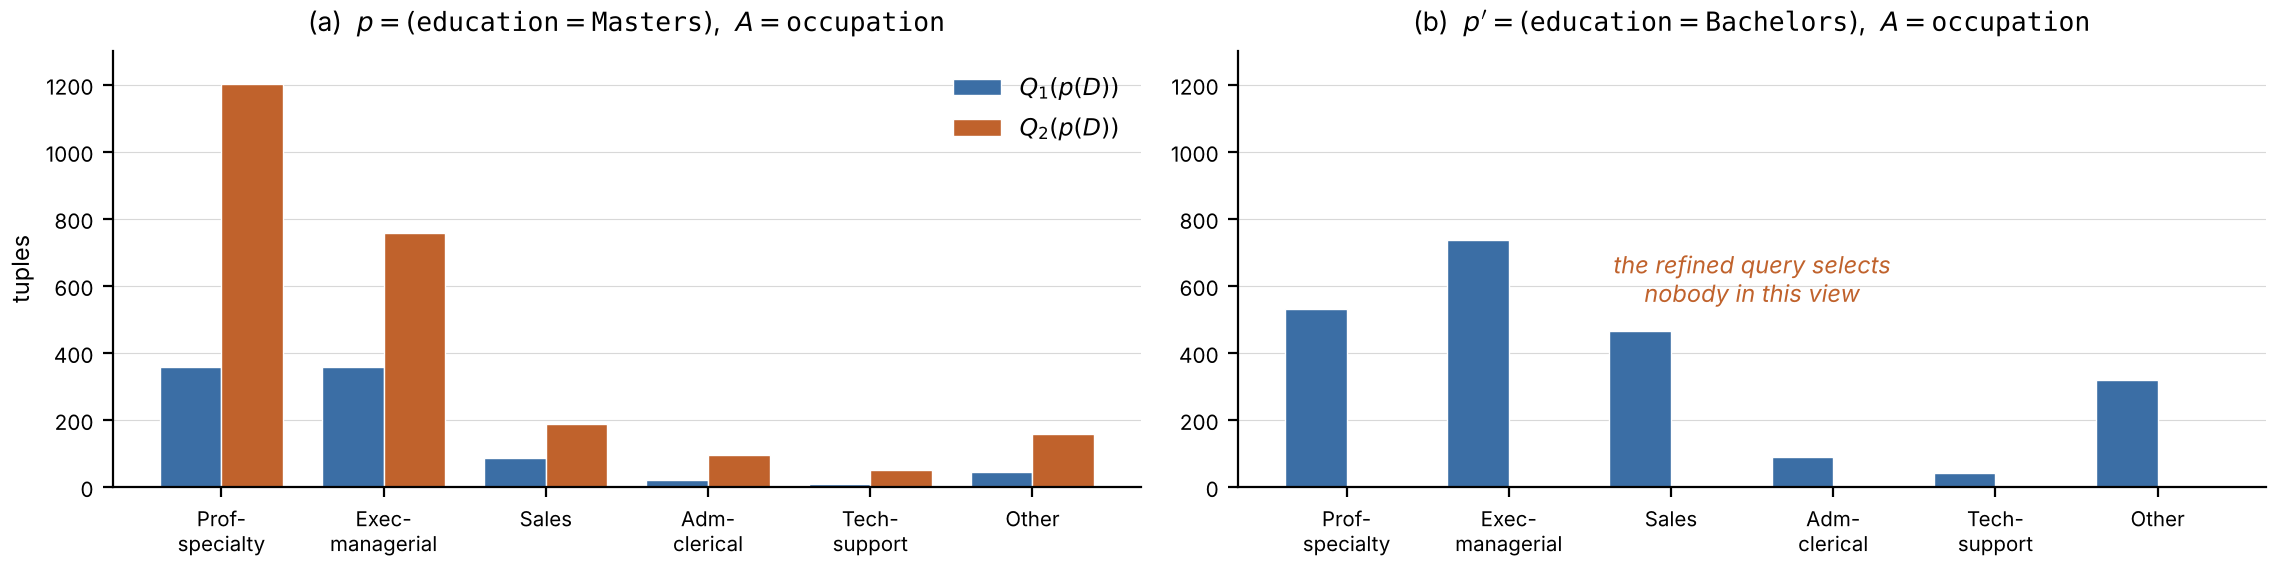
\includegraphics[width=\linewidth]{figures/candidates.png}
\caption{Two explanation candidates on Adult, for $Q_1$ selecting Bachelor's and Master's degree holders working at least $50$ hours and $Q_2$ selecting Master's degree holders working at least $30$ (Example~\ref{ex:candidate}). Counts are exact; what the framework releases is each pair of bars perturbed with Laplace noise.}
\label{fig:candidates}
\end{figure*}

What is released for a selected candidate is a perturbed version of its two histograms, in the sense of the Laplace mechanism (Definition~\ref{def:laplace-mechanism}).

\begin{definition}[Noisy histogram]
\label{def:noisy-histogram}
For a set of tuples $T\subseteq D$, an attribute $A$ and a scale $b>0$, the \emph{noisy histogram} of $A$ over $T$ is
\[
\hat H_{T,A}(v)=\hist{T}{A}(v)+Y_v,\qquad v\in\Dom(D[A]),
\]
with $Y_v$ drawn independently from the Laplace distribution of scale $b$, one draw per bin of the public domain of $A$.
\end{definition}

We release the pair $\big(\hat H_{Q_1(p(D)),A},\hat H_{Q_2(p(D)),A}\big)$ rather than only its difference, so that the analyst sees the two profiles themselves and not just the size of the gap between them.
The pair costs more: a tuple selected by both queries changes both histograms, so the pair has $L_1$-sensitivity $2$ against $1$ for the difference (Proposition~\ref{prop:histogram-release-sensitivity}), which doubles the noise scale at a fixed budget.
Where budget is scarce the difference can be released instead.
\alon{Done: a noisy histogram is now defined (Definition~\ref{def:noisy-histogram}); the paragraph that followed it has been cut to the two things it needs to say, what is released and what it costs, with the forward reference to the example removed.}



\subsection{Measures of Explanation Quality}
\label{sec:explanation-quality}

The criteria we optimise are the four reviewed in Section~\ref{subsec:prelim-quality}: interestingness, representativeness, coverage and diversity.
None is new.
What is new is the form we give them, and the reason for the change is always the same: a measure whose value can be swung by one individual cannot be optimised under differential privacy at all, because the noise a private mechanism must add is calibrated to exactly that swing.
For each criterion we therefore recall the form used in prior work, say what goes wrong with it here, and give the form we use.
Section~\ref{subsec:ideal-sensitivity} states the effect of all four changes in one place.

\paragraph{Interestingness.}
In its distributional form a candidate is scored by the distance between the two distributions it induces~\cite{SeeDB,FEDEX}, which in our setting is the total variation distance between the conditional distributions of $A$ over $Q_1(p(D))$ and $Q_2(p(D))$, or twice it in the normalised form.
Two things go wrong.
It is undefined when one of the two outputs does not meet the view, which is exactly the case of the one-sided views of Example~\ref{ex:candidate}, where a refinement adds or removes a population wholesale.
And because it is a ratio over the output sizes, a single tuple can move it by half of its entire range, however large the database (Proposition~\ref{prop:sensitivity-itemized}).
We therefore compare the two outputs \emph{bin by bin in counts}, normalised by the size of the bin in the view rather than by the size of the outputs, and add a public constant $\gamma$ to each denominator.

\begin{definition}[Smoothed Histogram Distance]
\label{def:hd}
Given a dataset $D$, a view predicate $p$, an attribute $A$, two queries $Q_1,Q_2$, and a public smoothing constant $\gamma \ge 0$,
\begin{multline}
\HD_\gamma(D;p,A,Q_1,Q_2) = \\
\sum_{v\in \Dom(D[A])}
\frac{\big|\hist{\Qone(\pD)}{A}(v)-\hist{\Qtwo(\pD)}{A}(v)\big|}
     {\hist{\pD}{A}(v)+\gamma}
\label{eq:hd-definition}
\end{multline}
\end{definition}

Setting $\gamma=0$ recovers the unsmoothed score, in which case the sum must be restricted to bins with $H_{p(D),A}(v)>0$ to avoid division by zero.
For $\gamma>0$ no such restriction is needed: a bin absent from $p(D)$ is necessarily absent from $Q_1(p(D))$ and $Q_2(p(D))$ as well, since both are subsets of $p(D)$, so it contributes exactly $0/\gamma=0$.

The motivation for $\gamma$ is a mismatch between the \emph{worst case} the sensitivity bound must cover and the \emph{typical case} the mechanism actually encounters.
A bin containing two tuples can have its ratio swung by a full unit by a single individual, so the unsmoothed bound must accommodate that; yet the bound is then applied uniformly, including to candidates supported by thousands of tuples.
The exponential mechanism consequently cannot separate candidates whose scores differ by far less than the bound.
Smoothing raises every denominator by a fixed public amount, which barely perturbs well-supported bins while removing the pathological ones from consideration.

The resulting bound is strictly decreasing in $\gamma$, which is the entire point: $\gamma$ buys a tighter worst case at the cost of a mild, uniform compression of every candidate's score.
The same device appears in differentially private decision-tree induction, where split criteria built from ratios of counts are smoothed for this reason~\cite{FriedmanSchuster10}, and in~\cite{DPClustX}, which rescales its cluster-quality measures by the cluster size; Section~\ref{subsec:prelim-dp} contrasts it with calibrating noise to the data instead.

\paragraph{Representativeness.}
Subgroup discovery scores a region by trading its unusualness against its generality~\cite{Wrobel97,HerreraCGJ11}; we need the requirement in the opposite direction, since the deviation we report is the change \emph{inside} a region and the region itself should be typical of the database.
The natural form is $1-\TVD$ between the distribution of an attribute inside the view and in the whole database.
Here too the view-side term $d_v/m$ is a ratio whose denominator is the view size, so a single tuple can rewrite the profile of a near-empty view (Proposition~\ref{prop:sensitivity-itemized}), and the measure is undefined when the view is empty.
The same smoothing repairs both.

\begin{definition}[Smoothed Representativeness]
\label{def:rep}
Let $c^A_v$ and $d^A_v$ be the number of tuples with $A$-value $v$ in $D$ and in $p(D)$, let $N=|D|$ and $m=|p(D)|$, and let $\gamma_R\ge0$ be a public constant.
For a single attribute,
\begin{equation}
\Rep^A_{\gamma_R}(p,D)=1-\frac{1}{2}\sum_{v\in\Dom(D[A])}\left|\frac{c^A_v}{N}-\frac{d^A_v}{m+\gamma_R}\right| ,
\label{eq:representativeness-proxy}
\end{equation}
and the representativeness of the view is the average over the reference attributes it does not itself constrain,
\begin{equation}
\Rep_{\gamma_R}(p,D)=\frac{1}{|\mathcal{A}_R(p)|}\sum_{A\in\mathcal{A}_R(p)}\Rep^A_{\gamma_R}(p,D),
\label{eq:rep-average}
\end{equation}
where $\mathcal{A}_R(p)=\mathcal{A}_R\setminus\mathrm{attr}(p)$.
\end{definition}

Two conventions are fixed by Eq.~\eqref{eq:rep-average}.
The reference set $\mathcal{A}_R$ is chosen in advance and does not depend on the candidate attribute, since representativeness is a property of the view and is evaluated before views are paired with attributes.
And the attributes the view itself constrains are excluded, because comparing $p(D)$ with $D$ on the attribute that defines $p$ is close to tautological: a view $\texttt{occupation}=c$ necessarily has an extreme occupation distribution.
We assume $|\mathcal{A}_R|>\ell$, so that $\mathcal{A}_R(p)$ is never empty.
We use $\gamma_R=N$ throughout; Section~\ref{subsec:two-stages} shows what that choice buys.
\ag{Is $\gamma_R$ a tunable argument or a fixed constant? The workflow paragraph lists it among the arguments of Algorithm~\ref{alg:main}, it is fixed to $N$ here, and every bound in this section is stated at $\gamma_R=N$. If it is always $N$, cleanest to drop it from the argument list. If it stays tunable, Eq.~\eqref{eq:rep-upper} and Proposition~\ref{prop:usefulness-sensitivity} should record that they hold at the default.}

Smoothing has a second, useful consequence: it bounds $\Rep_{\gamma_R}$ away from $1$, which the proof of Proposition~\ref{prop:usefulness-sensitivity} relies on.
The two vectors compared in Eq.~\eqref{eq:representativeness-proxy} do not carry the same total mass: the database side sums to $1$, while the view side sums to $m/(m+\gamma_R)$, which is below $1$ because smoothing inflates the denominator without adding to the counts.
Two non-negative vectors are at least as far apart in $L_1$ as their totals differ, so whatever the two profiles look like,
\[
\sum_v\Big|\tfrac{c_v}{N}-\tfrac{d_v}{m+\gamma_R}\Big|\;\ge\;1-\frac{m}{m+\gamma_R}\;=\;\frac{\gamma_R}{m+\gamma_R},
\]
and substituting this into Eq.~\eqref{eq:representativeness-proxy} gives
\begin{equation}
\Rep_{\gamma_R}(p,D)\;\le\;1-\frac{\gamma_R}{2(m+\gamma_R)}\;\overset{\gamma_R=N}{\le}\;\tfrac{3}{4},
\label{eq:rep-upper}
\end{equation}
the last step because $m\le N$ makes the fraction at least $\tfrac12$, and the average inherits the bound from the attributes it averages.
It is attained when the view is the whole database.

\paragraph{Coverage.}
A deviation seen on a handful of tuples is not evidence, and explanation frameworks pair a deviation measure with a mass measure: the support of association rules~\cite{AgrawalIS93}, the support threshold of MacroBase~\cite{MacroBase} and of \textsc{Diff}~\cite{DIFF}, the coverage of an anchor~\cite{Anchors}.
Since the object being explained is a comparison, the mass has to account for both outputs.
Taking the product of the two output sizes, as a two-sided support measure suggests, has the same defect as the distributional interestingness: it vanishes on one-sided views, and it grows with the size of the view, which is what makes a single tuple move it by an amount that grows with $N$ (Proposition~\ref{prop:sensitivity-itemized}).
\ag{Small issue: The sensitivity of the product is $o_1+o_2+1$, so it grows with the two output sizes, and the view size enters only as an upper bound on them. Saying it grows with the outputs would be more accurate.}
We take instead the evidence the two outputs place in the view \emph{jointly}, normalised by the public $N$:

\begin{equation}
\Cov(p,Q_1,Q_2,D)=\frac{|Q_1(p(D))|+|Q_2(p(D))|}{|D|}.
\label{eq:coverage-proxy}
\end{equation}
Dividing by $N$ costs nothing, since $N$ is public (Section~\ref{subsec:prelim-db-queries}), and it removes the growth with the database size: $\Cov$ reads as a fraction of the database rather than a count, so it is comparable across datasets and across views of very different sizes.
Its range is $[0,2]$, the upper end reached only when both outputs cover all of $D$, and it is $0$ exactly when neither output meets the view, which is the one case in which there is nothing to explain.
Summing rather than taking the smaller of the two counts matters for the same reason the sum replaces the product: a view that one output fills and the other leaves empty keeps the full weight of the evidence that is there.

\paragraph{Diversity.}
When several results are returned together their marginal value depends on what has already been shown, which is the principle of maximal marginal relevance~\cite{MMR} and of the axiomatic treatments that follow it~\cite{GollapudiS09,LinBilmes11}.
The aspect an explanation describes is its attribute, so we discourage reusing one, and grade the penalty by how many times it has already been used rather than charging every repeat alike:
\begin{equation}
\DivS(A,S)=\lambda^{\,\mathrm{count}(A,S)},
\qquad 0\le\lambda\le1,
\label{eq:diversity-score}
\end{equation}
where $\mathrm{count}(A,S)$ is the number of previously selected explanations already using attribute~$A$.
At $\lambda=1$ the term disappears and repeats are free; at $\lambda=0$ every repeat scores zero, which empties a candidate of value without removing it from the pool, so the mechanism may still return one.
Since $\DivS$ reads only previously selected \emph{outputs} and never the database, it adds no data sensitivity to the selection utility.

\paragraph{From a sequence to a set.}
Equation~\eqref{eq:diversity-score} is defined relative to the explanations chosen in earlier iterations, so as written it scores an \emph{ordered sequence}, not a set, while what we release is a set.
We therefore state the objective the algorithm approximates directly.

\begin{definition}[Set-level explanation utility]
\label{def:setobj}
Let $E$ be a set of candidates, and for an attribute $A$ let
$h^A_{(1)}\ge h^A_{(2)}\ge\cdots$ be the scores $\HD_\gamma(c)$ of the members of $E$ with $A_c=A$, in decreasing order.
For a non-increasing weight profile $w_1\ge w_2\ge\cdots\ge0$ with $w_1=1$,
\begin{equation}
F_w(E)=\sum_{A}\;\sum_{j\ge1} w_j\, h^A_{(j)} .
\label{eq:set-objective}
\end{equation}
\end{definition}
\ag{$A_c$ has not been introduced. Adding one clause to Definition~\ref{def:candidate}, writing $A_c$ for the attribute of a candidate $c$, fixes it here and in Proposition~\ref{prop:setobj}.}
\ag{The inner sum of Eq.~\eqref{eq:set-objective} has no upper limit, while $h^A_{(j)}$ exists only up to the size of the attribute group. Simplest fix is to adopt the convention $h^A_{(j)}=0$ for $j$ beyond the group.}

Within each attribute group the strongest explanation counts in full and every further one is discounted by its rank.
The graded penalty of Equation~\eqref{eq:diversity-score} is the profile $w_j=\lambda^{\,j-1}$, and a flat rule is $w=(1,\lambda,\lambda,\dots)$.
The two agree on the first two members of a group and differ only from the third onwards, so they can disagree about which set is best only when some attribute is used at least three times: that needs $k\ge3$, and once $k>2|\Attrs|$ it is unavoidable.

\begin{proposition}[The set objective agrees with the sequential rule]
\label{prop:setobj}
Order $E$ arbitrarily and write $S_{<c}$ for the members preceding $c$, so that the per-round rule of Eq.~\eqref{eq:diversity-score} awards $E$ the total $\sum_{c\in E}\HD_\gamma(c)\cdot\DivS(A_c,S_{<c})$.
With $w_j=\lambda^{\,j-1}$, $F_w(E)$ equals that total under the ordering maximising it, and upper-bounds it under every ordering.
\end{proposition}

\begin{proof}
Since $\mathrm{count}(A,S)$ counts only the members of $S$ that carry $A$, the weight a candidate receives depends on its position within its own attribute group and not on how the groups are interleaved.
The total therefore splits into independent per-group totals, and an ordering is free to choose each group's internal order.
Within the group of $A$, an ordering that places a member $j$-th awards it $\lambda^{\,j-1}$, so the group total is $\sum_j \lambda^{\,j-1}h_{\sigma(j)}$ for the induced permutation $\sigma$.
The weights are non-increasing, so by the rearrangement inequality this is maximised by pairing the largest weight with the largest score, that is by visiting the group in decreasing $\HD_\gamma$, and the maximum is $\sum_j \lambda^{\,j-1}h^A_{(j)}$.
Summing over groups gives Eq.~\eqref{eq:set-objective}, and no ordering gives more.
The special cases $\lambda=0$ and $\lambda=1$ recover a group maximum and a modular sum respectively.
\end{proof}
\alon{Done: Definition~\ref{def:setobj} restated in the general weighted form. As previously written it was the flat profile $w=(1,\lambda,\lambda,\dots)$ while Eq.~\eqref{eq:diversity-score} is the graded one $\lambda^{j-1}$; the two differ from the third member of a group onwards, so the equivalence claimed for them did not hold whenever an attribute was used three or more times.}

Set objectives of this shape are the ones greedy selection is usually defended for, by the $(1-1/e)$ guarantee of~\cite{NemhauserWF78}.
For $F_w$ a stronger statement holds, which we establish in Appendix~\ref{app:greedy}: because $F_w$ decomposes over attribute groups with no interaction between them, greedy is not a constant-factor approximation but returns the \emph{exact} maximiser, and the per-round score of Algorithm~\ref{alg:topk} is precisely its marginal gain.
\ag{The $(1-1/e)$ guarantee requires $F_w$ to be monotone submodular, which is now proved only in the appendix, so the reader meets the guarantee before the hypothesis. Please add one sentence recording that $F_w$ is monotone submodular, with a pointer to the appendix, closes the gap.}

\subsection{Sensitivity of the Measures}
\label{subsec:ideal-sensitivity}

Private selection with the exponential mechanism (Definition~\ref{def:exponential-mechanism}) calibrates its randomness to the global sensitivity of the utility (Definition~\ref{def:global-sensitivity}).
All statements are with respect to the unbounded neighbouring relation of Definition~\ref{def:neighboring}.
For a function $f$ and a size $N$ we write $\GS_N(f)$ for the largest change of $f$ between a database of size $N$ and a neighbour, so that $\GS(f)=\sup_N\GS_N(f)$; here $N$ ranges over all database sizes.
\ag{This sentence is dense. Two things would help. The clause after the semicolon repeats what the supremum already says and can go. And it is worth stating that a neighbour of a database of size $N$ has size $N+1$ or $N-1$, since that asymmetry is exactly what the two cases of Proposition~\ref{prop:usefulness-sensitivity} turn on.}
A mechanism running on the private database may calibrate to $\GS_N(f)$ at $N=|D|$ only if the size of $D$ is treated as public, as Section~\ref{sec:solution} does; otherwise it must calibrate to $\GS(f)$, since the scale of its noise would itself reveal $|D|$.
\ag{Publicity of $|D|$ is necessary here but it is not sufficient. Under Definition~\ref{def:neighboring} a neighbouring pair has $|D|=N$ and $|D'|=N+1$, so a mechanism that takes its scale from $|D|$ runs the exponential mechanism at two different temperatures on the two databases, whereas the usual $e^{\epsilon}$ argument needs one common scale. Two possible fixes. Either adopt the bounded relation, where $N$ is genuinely constant across the pair, or fix the scale from a public $\bar N$ that does not depend on $D$.}
Upper bounds below hold for every candidate; lower bounds and equalities are attained by explicit databases, and so require that the view and the two queries admit the tuples those databases use.
We begin with the one bound that takes real work, the smoothed Histogram Distance, and then state all four results together.

\begin{proposition}[Sensitivity of Smoothed Histogram Distance]
\label{prop:hd-sensitivity}
$\GS(\HD_\gamma)=\dfrac{1}{1+\gamma}$.
\end{proposition}

\begin{proof}
Let $D'=D\cup\{t\}$.
If $t$ does not satisfy $p$ nothing changes.
Otherwise $t$ falls into exactly one bin $v^*$ of $A$, and every other term of Eq.~\eqref{eq:hd-definition} is unchanged, so only that term has to be bounded.
Write $n=\hist{\pD}{A}(v^*)$ for the support of the view in that bin and $q_j=\hist{Q_j(\pD)}{A}(v^*)$ for $j=1,2$ for the two output counts in it, and let $n'=\hist{p(D')}{A}(v^*)$ and $q_j'=\hist{Q_j(p(D'))}{A}(v^*)$ be the same quantities on $D'$.
The numerators of the term before and after are $x=|q_1-q_2|$ and $x'=|q_1'-q_2'|$; since $Q_j(\pD)\subseteq\pD$ by Proposition~\ref{prop:view-restriction}, $0\le x\le n$.
Each query either selects $t$ or not, so $q_j'=q_j+\delta_j$ with $\delta_j\in\{0,1\}$, and $n'=n+1$ because $t$ satisfies $p$ and falls in $v^*$.
Substituting these,
\[
x'=|q_1'-q_2'|=\big|(q_1+\delta_1)-(q_2+\delta_2)\big|=\big|(q_1-q_2)+(\delta_1-\delta_2)\big| ,
\]
whereas $x=|q_1-q_2|$.
Both $x$ and $x'$ are absolute values, so by the reverse triangle inequality their difference is at most the absolute value of the difference of their arguments:
\[
|x'-x|\;\le\;\big|\,[(q_1-q_2)+(\delta_1-\delta_2)]-(q_1-q_2)\,\big|\;=\;|\delta_1-\delta_2|\;\le\;1 ,
\]
the last step because $\delta_1,\delta_2\in\{0,1\}$.
The term therefore moves from $x/(n+\gamma)$ to $x'/(n+1+\gamma)$.
If $n=\gamma=0$ the bin enters the sum with value $x'\le1=\frac{1}{1+\gamma}$.
\ag{One sentence here: At $\gamma=0$ this bin is excluded from the sum on $D$ by the restriction stated after Definition~\ref{def:hd} and included on $D'$, so the comparison is between a term that is absent and a term that is present. As written it reads as though the bin sat in both sums.}
Otherwise put $K=(n+\gamma)(n+1+\gamma)>0$ and bound the two directions separately.
Upwards, using in turn $x'\le x+1$, a common denominator, the cancellation of $xn+x\gamma$, then $x\ge0$ and $n\ge0$:
\begin{align*}
\frac{x'}{n+1+\gamma}-\frac{x}{n+\gamma}
&\;\le\;\frac{x+1}{n+1+\gamma}-\frac{x}{n+\gamma}\\[2pt]
&\;=\;\frac{(x+1)(n+\gamma)-x(n+1+\gamma)}{K}\\[2pt]
&\;=\;\frac{n+\gamma-x}{K}\\[2pt]
&\;\le\;\frac{n+\gamma}{K}\;=\;\frac{1}{n+1+\gamma}\\[2pt]
&\;\le\;\frac{1}{1+\gamma}.
\end{align*}
Downwards, using in turn $x'\ge x-1$, a common denominator, the same cancellation, then $x\le n$ and the step $(\star)$ below:
\begin{align*}
\frac{x}{n+\gamma}-\frac{x'}{n+1+\gamma}
&\;\le\;\frac{x}{n+\gamma}-\frac{x-1}{n+1+\gamma}\\[2pt]
&\;=\;\frac{x(n+1+\gamma)-(x-1)(n+\gamma)}{K}\\[2pt]
&\;=\;\frac{x+n+\gamma}{K}\\[2pt]
&\;\le\;\frac{2n+\gamma}{K}\\[2pt]
&\;\overset{(\star)}{\le}\;\frac{1}{1+\gamma}.
\end{align*}
Step $(\star)$ is the only one that is not immediate.
It asserts $(2n+\gamma)/K\le 1/(1+\gamma)$.
Since $K>0$ and $1+\gamma>0$, cross-multiplying preserves the inequality, so the claim is equivalent to $K-(2n+\gamma)(1+\gamma)\ge0$.
Expanding both products,
\begin{align*}
(2n+\gamma)(1+\gamma)&=2n+2n\gamma+\gamma+\gamma^2,\\[2pt]
K=(n+\gamma)(n+1+\gamma)&=n^2+n+2n\gamma+\gamma+\gamma^2 .
\end{align*}
The terms $2n\gamma+\gamma+\gamma^2$ occur in both lines and cancel, leaving $n^2+n$ from the second and $2n$ from the first, so
\[
K-(2n+\gamma)(1+\gamma)=(n^2+n)-2n=n(n-1),
\]
which is non-negative for every integer $n\ge0$, vanishing only at $n=0$ and $n=1$.
Equality holds for a bin holding one tuple of the view selected by $Q_1$ only, whose term is $\frac{1}{1+\gamma}$: adding a tuple of the same bin selected by $Q_2$ only makes the two counts equal and the term $0$.
\end{proof}

Step $(\star)$ is an equality exactly when $n(n-1)=0$, that is for $n\in\{0,1\}$: a bin the new tuple populates from empty, or one already holding a single tuple of the view.
For $n\ge2$ the bound $(2n+\gamma)/\big((n+\gamma)(n+1+\gamma)\big)$ is strictly smaller, and it falls as $n$ grows.
The sensitivity is therefore dictated by the sparsest bins of any view, whereas the candidates that make good explanations rest on well-populated ones.
\alon{Done: the bound was $2/(1+\gamma)$, proved by splitting the single changed bin with the triangle inequality and charging $1/(1+\gamma)$ twice. Bounding that bin directly gives $1/(1+\gamma)$, and the proof now exhibits a case attaining it, so the constant is exact rather than an upper bound. The halved sensitivity is carried into Proposition~\ref{prop:selection-utility-sensitivity}, Algorithm~\ref{alg:topk} and the calibration of $\gamma$.}

\begin{proposition}[Sensitivity of the forms used in prior work]
\label{prop:sensitivity-itemized}
Let $N$ be the database size, and restrict attention to neighbouring databases on which the measure in question is defined.
\begin{enumerate}[label=(\roman*),leftmargin=*]
\item \emph{Interestingness.} The distributional form has $\GS\ge1$, half of its range $[0,2]$.
\item \emph{Representativeness.} The unsmoothed form $1-\TVD$ has $\GS_N\ge\frac12-\frac1N$.
\item \emph{Coverage.} The two-sided support $|Q_1(\pD)|\,|Q_2(\pD)|$ has $\GS_N=2N+1$.
\end{enumerate}
None of the three decays with $N$, and the last grows with it.
\end{proposition}

\begin{proof}
(i) The score is twice a total variation distance and so lies in $[0,2]$.
Let $Q_1(\pD)=\{t\}$ with $t[A]=v_1$, and let $Q_2(\pD)$ place all its mass on a bin $v_2\ne v_1$, so the two conditional distributions are point masses at $v_1$ and at $v_2$ and the score is $2$.
Add one tuple of the view, selected by $Q_1$ only and with $A$-value $v_2$: the first distribution becomes uniform on $\{v_1,v_2\}$ and the score drops to $1$.
The rest of $D$ is unconstrained, so a change of $1$ is available at every database size.

(ii) Let $D$ hold one tuple of the view carrying the value $v_1$ on every attribute of $\mathcal{A}_R(p)$, together with $N-1$ tuples outside the view carrying $v_2$.
The view distribution is then a point mass at $v_1$ while the database gives $v_1$ weight $\tfrac1N$, so the measure is $\tfrac1N$.
Adding one tuple of the view with value $v_2$ makes the view distribution uniform on $\{v_1,v_2\}$ and the measure $\tfrac{N+3}{2(N+1)}$.
The change is $\tfrac{N+3}{2(N+1)}-\tfrac1N$, which exceeds $\tfrac12-\tfrac1N$ because $\tfrac{N+3}{2(N+1)}>\tfrac12$.

(iii) Write $o_j=|Q_j(\pD)|$ for $j=1,2$; by Proposition~\ref{prop:view-restriction} both are at most $m=|\pD|\le N$.
A tuple of the view selected by both queries sends $o_1o_2$ to $(o_1+1)(o_2+1)$, a change of
\[
(o_1+1)(o_2+1)-o_1o_2=o_1+o_2+1\;\le\;2N+1 .
\]
Equality holds at $o_1=o_2=m=N$, that is when the view is the whole database and both queries select all of it.
\end{proof}

\alon{Done: this proposition now states only the three lower bounds the prose of Section~\ref{sec:explanation-quality} cites it for. The upper bounds it used to carry for $\Cov$, $\Rep_{\gamma_R}$ and $\DivS$ were never cited anywhere: no mechanism consumes those measures on their own, only through $\Use$ (Proposition~\ref{prop:usefulness-sensitivity}) and $\widetilde{U}_i$ (Proposition~\ref{prop:selection-utility-sensitivity}), both of which derive what they need. The definedness claims are dropped as well, since each measure's paragraph above already makes them. The view-weighted product is dropped because no prior work proposes it.}

\subsection{The Two-Stage Model}
\label{subsec:two-stages}

A single private selection over $\mathcal{C}$ would have to score every candidate, and scoring a candidate means building the histograms of its attribute over both outputs inside its view.
That is $|\views|\cdot|\Attrs|$ pieces of work, repeated in each of the $k$ selection rounds.
Most of it is wasted: representativeness and coverage depend on the view alone, so whether a region can support an explanation at all can be decided before any attribute is looked at.
The framework therefore splits the problem in two.
The \emph{view stage} scores each view by the product of the two region-level measures,
\begin{equation}
\Use(p,Q_1,Q_2,D)= \Rep_{\gamma_R}(p,D)\cdot \Cov(p,Q_1,Q_2,D),
\label{eq:usefulness-proxy}
\end{equation}
with $\Rep_{\gamma_R}$ from Definition~\ref{def:rep} and $\Cov$ from Eq.~\eqref{eq:coverage-proxy}, and retains the $\tau$ best.
The \emph{explanation stage} then scores only the candidates built from the retained views, by the product of the two candidate-level measures:
\begin{equation}
\widetilde{U}_i(D;c)=\HD_{\gamma}(D;p,A,Q_1,Q_2)\cdot \DivS(A,S_{i-1})
\label{eq:selection-utility}
\end{equation}
for a candidate $c=(p,A)$.
\ag{The workflow paragraph and Figure~\ref{fig:framework} say $\gamma$ is refreshed each round from the accountant, so this utility and Proposition~\ref{prop:selection-utility-sensitivity} are really stated for the round's $\gamma_i$. Suggest carrying the index here, or adding a clause that the bound holds for whichever $\gamma$ the round uses.}
This reduces the candidate-level work from $|\views|\cdot|\Attrs|$ to $\tau\cdot|\Attrs|$, a factor $|\views|/\tau$, in every round.

Efficiency is the visible reason for the split, but not the binding one.
A single-stage mechanism would have to select on the product of all four measures, and a product is worse than its factors: by the product rule its sensitivity picks up a term in which the movement of one factor is multiplied by the \emph{level} of the other, and the levels here are not small.
Coverage alone can reach $2$, so an interestingness score that moves by $\Delta$ drags the combined score by $2\Delta$ before the coverage term is even counted.
Splitting removes that cross term entirely.
Each stage is its own private mechanism, calibrated to the sensitivity of its own utility, and neither pays for the other's range.
Propositions~\ref{prop:usefulness-sensitivity} and~\ref{prop:selection-utility-sensitivity} are what the two stages pay, and Section~\ref{subsec:dp-proof} composes them into $\epsilon$.

\begin{proposition}[Sensitivity of View Usefulness]
\label{prop:usefulness-sensitivity}
Treating $N=|D|$ as public and taking $\gamma_R=N$,
\[
\GS(\Use)\;\le\;\frac{9}{4N}.
\]
\end{proposition}
\ag{Notation. The bound depends on $N$, so the left-hand side should be $\GS_N(\Use)$ and not $\GS(\Use)$, which Section~\ref{subsec:ideal-sensitivity} defines as $\sup_N \GS_N$. The same issue appears in the filtering paragraph at the end of this section. A one-symbol fix, and it preserves the distinction drawn above.}

\begin{proof}
Write $\Use=\Rep_{\gamma_R}\cdot\Cov$, let $m=|p(D)|$ and $K=(m+\gamma_R)(m+1+\gamma_R)$.
The product rule gives
\begin{equation}
|\Use(D)-\Use(D')| \;\le\; \Delta\Rep\cdot\Cov(D) + \Rep(D')\cdot\Delta\Cov .
\label{eq:usefulness-product-rule}
\end{equation}

\emph{Second term.} One tuple may satisfy both $Q_1$ and $Q_2$, so it changes $|Q_1(p(D))|+|Q_2(p(D))|$ by at most $2$ and $\Delta\Cov\le 2/N$.
\ag{The bound is right, but the details are incomplete, since $\Cov$ has $|D|$ in its denominator and that moves as well. Writing $s'=s+\delta$ with $\delta\le2$ gives $|\Delta\Cov|=|\delta N-s|/(N(N+1))\le 2/(N+1)$, which is what we need and is consistent with the out-of-view case below.}
By Eq.~\eqref{eq:rep-upper}, $\Rep\le\tfrac34$, so this term is at most $\tfrac32\cdot\tfrac1N$.

\emph{First term, tuple inside the view.} Suppose the tuple satisfies $p$ and lands in bin $v^*$, so that $c_{v^*}$ and $d_{v^*}$ each increase by $1$ and $m$ becomes $m+1$.
Writing $e_v=c_v/N-d_v/(m+\gamma_R)$ for the $v$-th summand,
\[
e_v'-e_v=\frac{d_v}{K}\quad(v\ne v^*),
\qquad
e_{v^*}'-e_{v^*}=\frac1N-\frac{m+\gamma_R-d_{v^*}}{K}.
\]
\ag{These two movements fix the values of $N$ and $\gamma_R$ on $D$, but the neighbor has $|D'|=N+1$ and therefore $\gamma_R'=N+1$, so the true summands are $c'_v/(N+1)-d'_v/(m+N+2)$. The out-of-view case below does let $\gamma_R$ rise, and the $\gamma_R=0$ discussion after Remark~\ref{rem:usefulness-tightness} has a $2/(N+1)$ term for this change, so the subsection currently uses three different conventions. Please Rewrite this case. A numerical search with both quantities moving gives $\sup N|\Delta\Use|=3/2$ for a tuple inside the view and $7/4$ for one outside it, so $9/(4N)$ is kept and the true constant is $7/(4N)$.}
The two contributions at $v^*$ carry \emph{opposite} signs and therefore partially cancel, which is what the following bound retains:
\[
\Delta\Rep\;\le\;\tfrac12\left[\frac{m-d_{v^*}}{K}+\left|\frac1N-\frac{m+\gamma_R-d_{v^*}}{K}\right|\right].
\]
Multiplying by $\Cov\le 2m/N$ and maximising over $0\le d_{v^*}\le m$ and $0\le m\le N$ with $\gamma_R=N$, the maximum is attained at $m=N$ and equals $\tfrac34\cdot\tfrac1N$.

Adding the two terms gives $\tfrac32\cdot\tfrac1N+\tfrac34\cdot\tfrac1N=\tfrac94\cdot\tfrac1N$.

\emph{Tuple outside the view.} This case needs its own treatment, because $\Cov$ is \emph{not} unchanged: its numerator is, since a tuple outside the view joins neither $Q_1(p(D))$ nor $Q_2(p(D))$, but its denominator $|D|$ grows.
Here the sum in Eq.~\eqref{eq:representativeness-proxy} collapses.
Every summand is non-negative, since $d_v\le c_v$ and $m+\gamma_R\ge N$ give $d_v/(m+\gamma_R)\le c_v/N$, so the absolute values can be dropped and
\[
\sum_v\Big(\frac{c_v}{N}-\frac{d_v}{m+\gamma_R}\Big)=1-\frac{m}{m+\gamma_R},
\]
which depends on $m$ alone and not on which bin the new tuple joined.
With $m$ and $d$ fixed and $\gamma_R=N$ rising to $N+1$, this gives the \emph{exact} movement $\Delta\Rep=-\tfrac12\,m/K'$ with $K'=(m+N)(m+N+1)$, and $\Rep=\tfrac12+m/(2(m+N))$.
Writing $s=|Q_1(p(D))|+|Q_2(p(D))|\le 2m$, the two coverages are $s/N$ and $s/(N+1)$, so
\[
|\Delta\Use| = s\left[\frac{\Rep}{N(N+1)}+\frac{m}{2K'(N+1)}\right]
\;\le\;\frac{7}{4(N+1)},
\]
using $s\le2m\le2N$, $\Rep\le\tfrac34$ and $K'\ge N(N+1)$.
\ag{The constant is correct, but these three bounds applied independently yield roughly $5/(2(N+1))$. Getting $7/4$ needs $s\,m/K'$ maximised jointly, and since both bracketed terms increase in $m$ it is enough to evaluate at $m=N$, where $K'=2N(2N+1)$ and the second term is $N/(2(2N+1)(N+1))$, tending to $1/(4(N+1))$. I suggest replacing the justification with this observation.}
Since $\tfrac74<\tfrac94$, the in-view case governs and the stated bound stands.
\ag{The wording reads as if the in-view case were the worst case, which is the reverse of what Remark~\ref{rem:usefulness-tightness} and the numbers say. I suggest stating that the in-view bound is the larger of the two and therefore fixes the constant we claim, while the best lower bound we have comes from the out-of-view case. That also removes the clash with the note after the remark, which says the out-of-view case attains the maximum.}

The argument above is stated for a single attribute; since $\Rep_{\gamma_R}$ is the \emph{average} over $\mathcal{A}_R$ of quantities each obeying the same bound, and an average cannot exceed the maximum, the bound carries over unchanged.

The assumption that $N$ is public is necessary and is stated explicitly: $\Cov$ is a ratio whose denominator is itself data-dependent, so without it no constant bound independent of the database size exists.
\end{proof}

\begin{remark}[Tightness]
\label{rem:usefulness-tightness}
The bound is not tight, and the gap is at most a factor of $9/7$.
For the lower bound, let every tuple of $D$ satisfy $p$ and be selected by both queries.
The view is then the whole database, so $\Rep_{\gamma_R}$ sits at its ceiling $\tfrac34$ and $\Cov=2$, giving $\Use=\tfrac32$.
Add one tuple outside the view, in a bin of $A$ that $D$ does not yet use.
No count inside the view changes, but $|D|$ does, and by the computation in the proof above
\[
|\Delta\Use|=\frac{3}{2(N+1)}+\frac{N}{2(2N+1)(N+1)}\;\xrightarrow[N\to\infty]{}\;\frac{7}{4(N+1)} ,
\]
so the true constant lies in $[7/4,\,9/4]$.
The remaining slack is in the in-view case, where the two terms of Eq.~\eqref{eq:usefulness-product-rule} are bounded separately at $m=N$: at that point $\Cov=2$ forces $Q_1$ and $Q_2$ to cover the whole database, which in turn forces $d_v=c_v$ and makes $\Delta\Rep$ far smaller than the bound used.
Exploiting that coupling would close the remaining factor; we have not carried it out.
\ag{This can be sharpened. The in-view case, computed with $N$ and $\gamma_R$ both moving, maxes out at $3/2$, below $7/4$, so the out-of-view construction is at once the lower bound and the global maximum and the interval collapses to $7/4$. We can therefore state Proposition~\ref{prop:usefulness-sensitivity} as $7/(4N)$ as soon as the in-view case is bounded below $7/4$, which it is with room to spare, and no coupling argument is needed.}
\end{remark}

\alon{Done: the earlier statement claimed $2/N$ with a proof that bounded only $\Delta\Cov$ and treated $\Rep$ as a fixed multiplier, omitting the $\Delta\Rep\cdot\Cov$ term entirely, which the construction of Remark~\ref{rem:usefulness-tightness} already violates. Representativeness is now smoothed by $\gamma_R$, which both fixes the sensitivity and stabilises the constant in $N$, and the corrected bound $9/(4N)$ is proved above, with a matching lower bound of $7/(4N)$ in Remark~\ref{rem:usefulness-tightness}. The proof now also covers the case of a tuple outside the view, which the earlier version dismissed and which is in fact the one that attains the maximum.}

The constant $9/4$ is the reason representativeness is smoothed at all.
Repeating the proof with $\gamma_R=0$ costs on both terms.
Eq.~\eqref{eq:rep-upper} degenerates to $\Rep\le1$, so the term $\Rep\cdot\Delta\Cov$ grows from $\tfrac32\cdot\tfrac1N$ to $2/N$; and the view-side movement is no longer damped, so $\Delta\Rep\le\tfrac12\big(\tfrac{2}{N+1}+\tfrac1{m+1}\big)$ against $\Cov\le2m/N$ gives roughly $3/N$ at $m=N$ in place of $\tfrac34\cdot\tfrac1N$.
Smoothing also buys the structure the second case of the proof rests on: with $\gamma_R=0$ the summands of Eq.~\eqref{eq:representativeness-proxy} need not be non-negative, so the sum does not collapse and the exact movement is unavailable.
The unsmoothed product therefore admits only a bound near $5/N$, more than doubling the constant, and smoothing the view-side denominator is the one further change the split alone did not deliver.

\begin{proposition}[Sensitivity of the selection utility]
\label{prop:selection-utility-sensitivity}
$\GS(\widetilde{U}_i)\le 1/(1+\gamma)$.
\end{proposition}

\begin{proof}
Condition on the history $S_{i-1}$ of previously released outputs, which is legitimate under adaptive composition.
Given that history, $\DivS(A,S_{i-1})$ is a constant in $[0,1]$ determined entirely by released values, so it acts as a bounded multiplier on the data-dependent factor and cannot increase its sensitivity.
The claim follows from Proposition~\ref{prop:hd-sensitivity}.
\end{proof}

Filtering is not free.
The view stage ranks by $\Use$, which no explanation score enters, so a view of middling usefulness may host the single most interesting explanation and still be dropped; and because the filter itself is private, the retained set is not even the exact top-$\tau$ by $\Use$.
We do not bound what this costs.
The one-shot top-$\tau$ mechanism admits a high-probability utility guarantee whose slack grows as $\tau\Delta\log|\views|/\epsilon_P$, which at $\Delta=9/(4N)$ is $9\tau\log|\views|/(4N\epsilon_P)$ and so vanishes with the database size.
What that slack must be compared against, however, is not the scale of $\Use$ but the gap between the $\tau$-th and the $(\tau{+}1)$-th best view, and that gap narrows as the view space grows denser.
The guarantee is therefore informative only under a lower bound on the gap, which we do not assume.
What the form does say is that the cost of filtering grows linearly in $\tau$, which is an argument for keeping $\tau$ small.
\alon{TODO: a utility guarantee for the view stage is the main gap in Section~\ref{sec:model}. The honest statement today is the one above; quantifying it, either by a sharper analysis of the one-shot mechanism at small $\epsilon_P$ or by an assumption on the gap between the $\tau$-th and $(\tau{+}1)$-th views, would close it.}

\alon{Done: Section~\ref{sec:model} now presents each quality measure as a modification of the form used in prior work, isolates in one proposition the sensitivity of the forms used in prior work, and derives the two-stage split from the efficiency of filtering; the former Section~3.4 is absorbed here.}
